\documentclass{article}
\usepackage[utf8]{inputenc}

\title{DATA 780 Group Project: Waterflow \\ \large Midway Report}
\author{%
  Spencer Childress \\
  School of Data and Information Sciences \\
  University of North Carolina at Chapel Hill \\
  Chapel Hill, NC \\
  \texttt{spncr@unc.edu} \\
  \And
  Jay Patel \\
  School of Data and Information Sciences \\
  University of North Carolina at Chapel Hill \\
  Chapel Hill, NC \\
  \texttt{jmjay1@email.unc.edu} \\
  \And
  Ryan Willis \\
  School of Data and Information Sciences \\
  University of North Carolina at Chapel Hill \\
  Chapel Hill, NC \\
  \texttt{rywillis@unc.edu}
}
\date{\today}
% `preprint` shows author names (the default mode prints "Anonymous Author(s)")
\usepackage[preprint]{nips_2018}
\usepackage{graphicx}  % figures from docs/md/figures
\providecommand{\pandocbounded}[1]{#1}  % newer Pandoc wraps images in this
\providecommand{\tightlist}{%  % Pandoc emits this inside compact lists
  \setlength{\itemsep}{0pt}\setlength{\parskip}{0pt}}
% Keep figures where they appear in the text instead of floating to the end
\usepackage{float}
\floatplacement{figure}{H}
% nips_2018 sets \flushbottom, which stretches list/paragraph spacing on pages
% left short by an H figure; let short pages stay short instead
\raggedbottom

\begin{document}

\maketitle

\section{Introduction}\label{introduction}

We intend to build a machine learning model that predicts water flow in
water basins without sensor data. The inputs to the model include land,
soil and climate attributes, which will be evaluated against water flow
measurements from water basins with sensor data. Most water basins have
no sensor data yet water managers need flow estimates for flood and
drought planning. An inexpensive, interpretable method that can be
easily deployed where we have confidence in its predictive power is
useful, and understanding where the method fails improves our
understanding of hydrologic processes.

Today, hydrologists tune a physical model for each river with historical
measure water flow. For rivers without sensor data, they compare with
nearby, similar ``donor'' rivers, which has proven to be failure-prone.
Deep learning models trained on hundreds of rivers now do better
(Kratzert et al., 2019), but they're computationally intensive and
suffer from interpretability.

Our approach will test whether the standard practice that ``similar
rivers behave alike'' improves with unsupervised water basin clustering
and predictive models accounting for spatial proximity, weather
patterns, and ecological attributes. We will compare models with minimal
inputs, a basin's cluster, and its full attributes to determine the most
accurate approach. We want to understand the most predictive
characteristics, in particular whether basin clustering is an
informative exercise.

Clustering may discard important information from the raw attributes of
the water basins in the training data and predefined weather windows may
need additional context to account for slow snowmelt and groundwater
levels. However, clustering may help when training basins are scarce,
where informatively characterizing a water basin from its raw attributes
is impractical. Therefore, our main focus will be to evaluate whether
clustering helps when training basins are scarce.

We will assess our model on its predictive accuracy of water flow, as
measured with the Nash-Sutcliffe Efficiency metric:

\[
\mathrm{NSE} = 1 - \frac{\sum_{t} \left(Q_{\mathrm{obs},t} - Q_{\mathrm{pred},t}\right)^2}{\sum_{t} \left(Q_{\mathrm{obs},t} - \bar{Q}_{\mathrm{obs}}\right)^2}
\]

We will train separate neural networks for each cluster. New and test
observations will be assigned to the nearest cluster centroid and then
routed to the corresponding neural network for prediction. To avoid
leakage we will split by basin using spatially-blocked folds; refit
scalers PCA and clustering inside each fold; and train on earlier years
to avoid temporal correlation.

\section{Related Work}\label{related-work}

Previous research in this area for determining streamflow has used
several different models and traditionally they have been process based
models. These models are typically based on mathematical formulas that
are common in hydrological sciences but there is room for improvement as
they are by no means 100\% accurate. In our main research paper
reference (Kratzert et al., 2019) it is pointed out that machine
learning methods have come a long way and being data driven they take
into account more than the process based methods can. This is
particularly useful for hydrologically diverse catchments where process
based models typically need a deeper knowledge of a particular area
which can be expensive/time consuming.

In the past Machine Learning models have been used to measure streamflow
in ungauged basins even better than conceptual models that were
calibrated for each catchment. This is even against gauged basins that
are operating on a calibrated process model. While in the paper we
researched this was on an average basis (didn't outperform all
process/calibrated models), it does provide evidence that data based
models are effective. This is particularly important for ungauged basins
since even if financially hydrologists are able to start gauging the
basin it will take 2-3 years to get a reliable data set.

Previous machine learning models researched were a type of recurrent
neural network (RNN). They were specifically called Long short-term
memory (LSTM) networks. These were used because they are great for long
term models that look at weather effects that happen over time. They are
useful for things like snowfall accumulation and vegetation growth.
These happen over long lengths of time so it makes them useful for
modeling basin catchment. In the results of their study they observed
that LSTM network models using static catchment attributes was
determined to be the most useful. We will be using this add a reference
to see if we can create a machine learning model that is easier to
interpret as well as less intensive.

\section{Methods}\label{methods}

The dataset will be derived from the Caravan v1.6 CSV release,
specifically looking at US basins (camels), Great Britain basins
(camelsgb), and Australia basins (camelsaus), totaling 1760 basins.
Measurments for all basins will be daily from 1981-2014. Basins will be
kept for analysis based on overall quality and completeness.

Static attributes for the kept basins will represent the physical and
environmental characteristics of each basin. These attributes will be
standardized prior to clustering and model development, with all
preprocessing parameters estimated exclusively from the training
catchments within each validation fold.

To prevent information leakage, catchment attributes derived directly
from observed streamflow or other discharge-related measurements will be
excluded from the predictor set. The remaining static catchment
attributes will be examined for missing values, inconsistencies, and
potential redundancy before model development.

Meteorological predictors will be constructed using fixed time intervals
of 7, 30, 90, and 365 days. These intervals will capture short-term and
longer-term hydrological and climatic conditions that may influence
streamflow behavior, all of which will be applied consistently across
all models.

The target variable, daily streamflow, will be log-transformed to reduce
the influence of highly skewed flow distributions and improve model
stability. Predictions will subsequently be evaluated in both
transformed and original flow spaces to assess the implications of the
transformation and back-transformation procedure.

Prior to model fitting, basins will be split into training and test
sets. All preprocessing operations, including feature scaling and any
dimensionality reduction, will be fitted independently within each
training fold. This procedure will ensure that information from held-out
catchments does not influence model development.

The scope of this analysis will involve the usage of several machine
learning methods, both supervised and unsupervised. Ridge regression
will serve as a baseline supervised method, and it will be run on lagged
weather measurements and accuracy of nearest-gauge transfer.

After establishing a baseline ridge regression model, k-means clustering
will be applied to the static catchment attributes to identify groups of
physically similar river basins. Catchments will be classified into
groups based on their similarity across the selected standardized
attributes. The number of clusters (k) will be evaluated across three to
four candidate values. This will allow the study to examine whether the
granularity of catchment groupings influences predictive performance.
Once clustering is done, each catchment will be assigned a cluster
identifier. This identifier will subsequently serve as an alternative
representation of catchment characteristics in the supervised methods.

An important consideration is that cluster membership is derived
directly from the underlying catchment attributes. Consequently, cluster
identifiers do not introduce additional information beyond the original
attributes. Instead, they provide a potentially more parsimonious
representation of catchment similarity that may improve predictive
performance when the available training sample is small. The
hydrological coherence of the resulting clusters will also be examined
to determine whether catchments grouped together based on physical
characteristics demonstrate meaningful similarities in their observed
streamflow behavior.

Light Gradient Boosting Machine (LightGBM) will serve as the primary
supervised learning method for streamflow prediction. LightGBM is a
gradient-boosted decision tree framework that can accommodate nonlinear
relationships and interactions between meteorological and catchment
characteristics. For this model, 3 different configurations will be
compared to determine best performance: - No catchment information: The
model will use meteorological forcing variables without static catchment
attributes or cluster identifiers. - Cluster-based information: The
model will incorporate meteorological forcing variables and the
corresponding unsupervised cluster identifier derived from the k-means
clustering model. - Raw catchment attributes: The model will incorporate
meteorological forcing variables and the complete set of selected static
catchment attributes prior to log transformation.

\section{Preliminary Results}\label{preliminary-results}

To preface, we have only begun exploratory data analysis following the
finalization of our analysis plan, updated with the feasibility review
from Professor Chiang. With the decision made to exclude the water
basins out of Great Britain, our training and test data will be drawn
from the following regions:

\begin{itemize}
\tightlist
\item
  \texttt{camels}, a database of 671 US water basins, of which 631
  contain sufficient data
\item
  \texttt{camelsaus}, a database of 561 Australian water basins, of
  which 541 contain sufficient data
\end{itemize}

Below is a map of the basins available in the two databases.

\begin{figure}
\centering
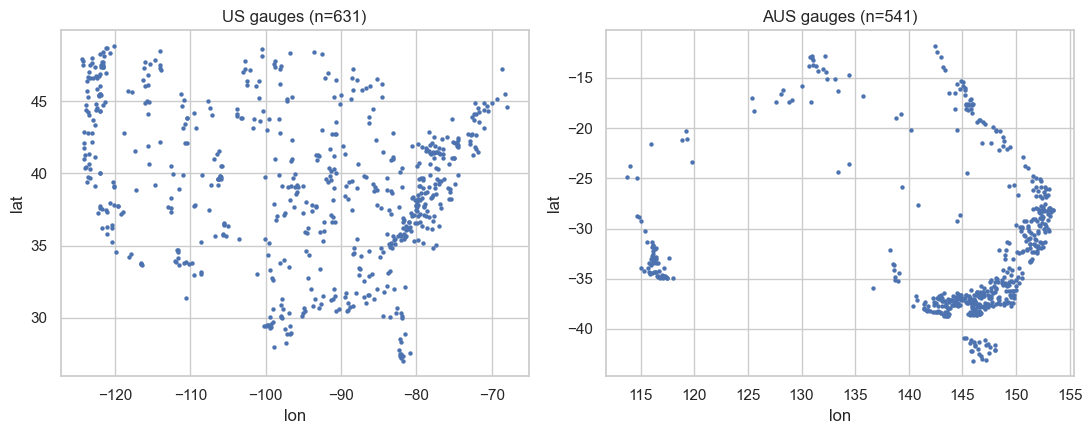
\includegraphics[width=1\linewidth,height=\textheight,keepaspectratio]{figures/basin-map.png}
\caption{Map of the basins available in the \texttt{camels} and
\texttt{camelsaus} databases.}\label{fig:basin-map}
\end{figure}

To arrive at the set of water basins with sufficient data we applied the
following thresholds:

\begin{itemize}
\tightlist
\item
  At least 15 years of valid water flow data.
\item
  At most 15\% of missing window days.
\end{itemize}

The following figures provide comparisons of the two databases.

\begin{figure}
\centering
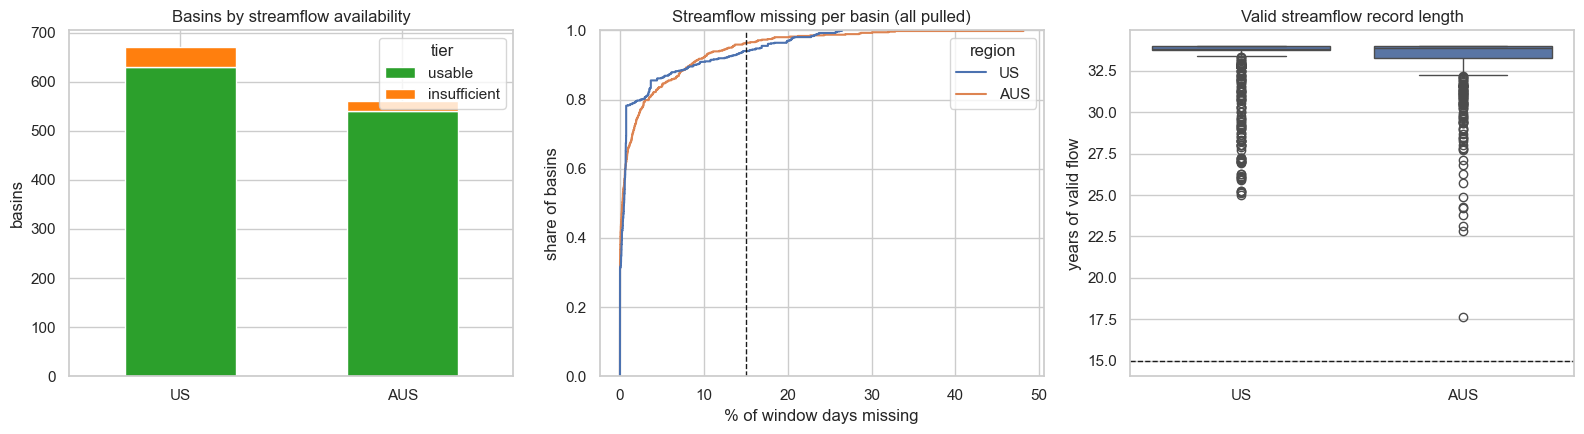
\includegraphics[width=1\linewidth,height=\textheight,keepaspectratio]{figures/region-comparison.png}
\caption{Comparison of the \texttt{camels} and \texttt{camelsaus}
databases.}\label{fig:region-comparison}
\end{figure}

Below we dril down into the availability of streamflow data over time,
from the early 1980s to the mid 2010s.

\begin{figure}
\centering
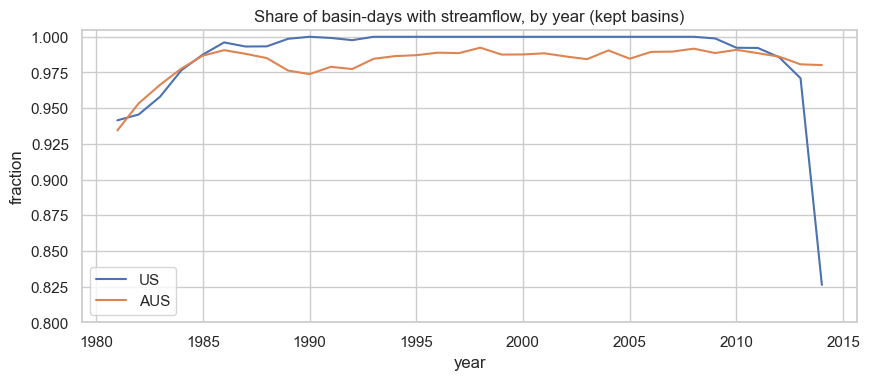
\includegraphics[width=1\linewidth,height=\textheight,keepaspectratio]{figures/missingness-by-year.png}
\caption{Availability of streamflow data by
year.}\label{fig:missingness-by-year}
\end{figure}

To get an idea of the data present for each basin, we zoom in below on a
single basin.

\begin{figure}
\centering
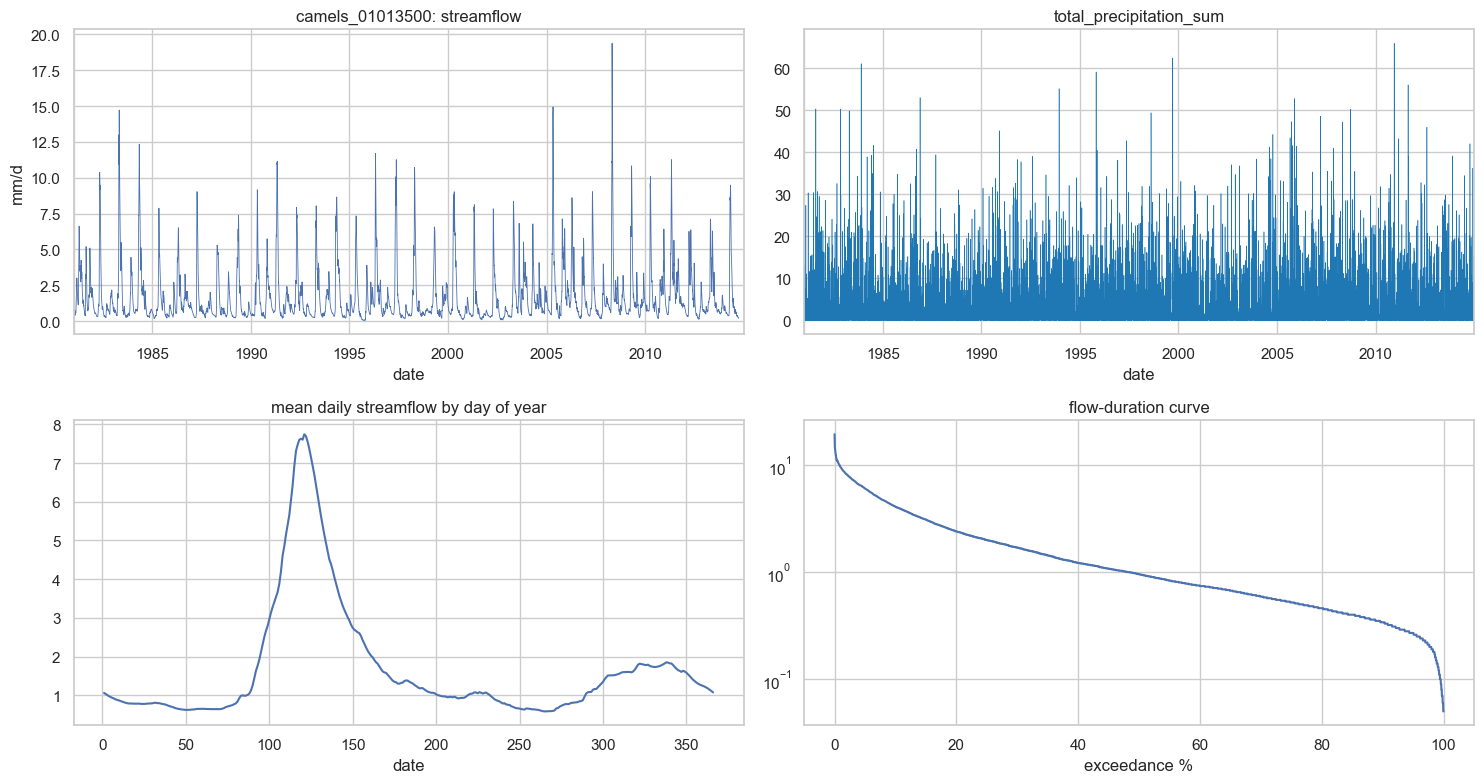
\includegraphics[width=1\linewidth,height=\textheight,keepaspectratio]{figures/example-basin.png}
\caption{Streamflow data for a single example
basin.}\label{fig:example-basin}
\end{figure}

Note the seasonal spikes \textasciitilde120 days into the year where
waterflow rises following spring precipitation. Our immediate next steps
are to define the temporal split of our training and test data, and the
locational blocking of our water basins, to inform k-fold validation.

\section{Future Plans}\label{future-plans}

The remaining work will focus on the leakage-safe US/AUS comparison and
whether cluster information helps when training basins are scarce. The
proposed milestones and division of labor are:

\begin{itemize}
\item
  \textbf{November 15 --- Scope and evaluation protocol:} Spencer leads
  scope and validation; Jay leads data and features; Ryan supports
  clustering and evaluation.
\item
  \textbf{November 22 --- Core experiments and results freeze:} Ryan
  leads LightGBM runs; Jay supports data and baselines; Spencer leads
  the basin-scarcity analysis.
\item
  \textbf{November 27 --- Results synthesis:} Spencer leads
  interpretation; Ryan provides model diagnostics; Jay verifies data and
  forcing caveats.
\item
  \textbf{November 29 --- Full paper draft:} Spencer integrates the
  paper; Jay drafts data and methods; Ryan drafts modeling and results.
\item
  \textbf{December 3 --- Revision and reproducibility:} Spencer leads
  revisions; Jay verifies data claims; Ryan runs the clean-environment
  check.
\item
  \textbf{December 6 --- Presentation and internal release:} Ryan
  prepares slides; Spencer and Jay review; all rehearse.
\item
  \textbf{December 7--9 --- Final quality checks:} All review
  compilation, wording, and submission requirements; Spencer
  coordinates.
\item
  \textbf{December 10 --- Final report submission:} Spencer coordinates;
  all confirm the final files and results.
\end{itemize}

Optional work (synthetic benchmark, CAMELS-GB, cross-region transfer,
kernel regression, or expanded SHAP) will not delay the November 22
freeze; retain only a minimal synthetic positive control if the course
requires it and time permits.


\bibliographystyle{plainnat}
\bibliography{references}

\end{document}
